\section{Extended Related Work}
\label{sec:appdx-related-work}

SSD is complementary to other lines of work that accelerate LLM inference through orthogonal means: hardware-aware algorithms like FlashAttention \citep{Dao2022FlashAttention}, KV-cache management and paging \citep{kwon2023efficient,zhang2023h2o,Hooper2024KVQuant}, sparse or approximate attention \citep{Beltagy2020Longformer,Zaheer2020BigBird}, and multi-token or tree-based draft methods \citep{Cai2024Medusa,Fu2024Lookahead}. SSD targets a different bottleneck---the sequential dependence between drafting and verification---and can in principle be combined with any of these.

% \color{red}
\section{Combining SSD with SD Variants}
\label{app:combine}

\textbf{EAGLE-3.} EAGLE-3 \citep{eagle3} improves the acceptance rate $\alpha$ by training the draft to condition on target activations extracted during the previous round's verification. When target activations are unavailable mid-speculation, the draft conditions on its own activations as a surrogate, with acceptance degrading slowly as more self-generated activations are used.

This is entirely compatible with SSD, with one nuance: since the SSD draft begins speculating round $T{+}1$ pre-emptively, it does not yet have target activations from round $T$ (unlike standard EAGLE-3, which waits for them). With lookahead $K$, the draft thus conditions on up to $2K$ self-generated tokens, lowering acceptance on the latter $K$. This can be mitigated by training the EAGLE-3 draft to preserve acceptance over longer periods of self-conditioning. This is depicted in Figure~\ref{fig:eagle3-ssd}. 

\begin{figure}[h]
    \centering
    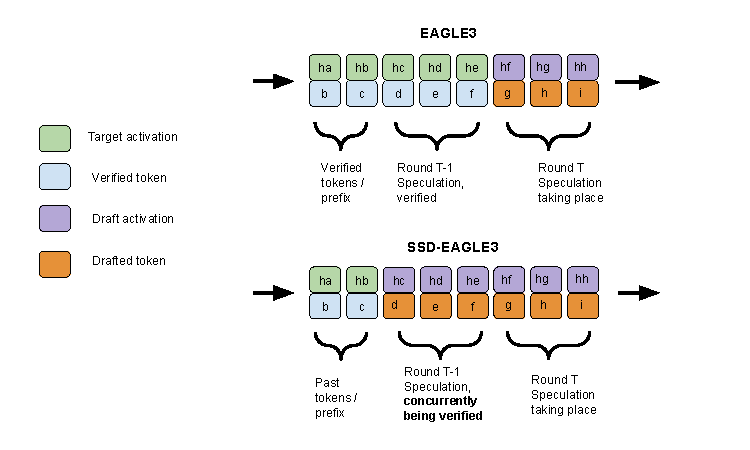
\includegraphics[width=0.85\linewidth]{figures/eagle3-figure.pdf}
    \caption{Comparison of activation conditioning in EAGLE-3 vs.\ SSD-EAGLE-3. In standard EAGLE-3 (bottom), the round $T$ draft conditions almost entirely on target activations extracted from the already-verified round $T{-}1$. In SSD-EAGLE-3 (top), round $T$ speculation begins \textit{before} round $T{-}1$ verification completes, so the draft must substitute its own activations (light nodes) for the not-yet-available target activations. Conditioning on more draft activations can degrade quality of EAGLE speculations if the draft model is not trained to use draft self-conditioning effectively.}
    \label{fig:eagle3-ssd}
\end{figure}

In our implementation, the target model sends the number of accepted tokens per sequence as well as the target activations at each relevant token position to the draft over NCCL for the draft model to condition on when speculating. 

\textbf{Token-Tree Methods.} 
Token-tree SD methods~\citep{specinfer,sequoia,eagle2,eagle3} can be combined naturally with SSD.
SSD drafts a linear chain for many possible verification outcomes.
To combine SSD with these token-tree approaches, one would simply pre-speculate (and verify) a token tree for each verification outcome instead of a token chain.
In practice, this requires a more elaborate attention mask than that presented in Figure \ref{fig:custom-mask}.


\color{black}